\singlespacing
\chapter{Microespectrómetro}
\label{chap:microsp}
\spacing{1.5}

\hspace{0.5cm}En este capítulo se describe el montaje y la caracterización de un microespectrómetro utilizado para caracterizar espectralmente los defectos del filtro.

The MSP is a hyphenated instrument that integrates a light microscope
with a UV–vis–NIR spectrophotometer. The spectrophotometer
measures the intensity of various wavelengths of light from the ultraviolet
through the visible and NIR regions. The microscope is an imaging tool
designed to enlarge an image of microscopic objects so that they may be studied
easily. Integrated as the UV–vis–NIR MSP, such a device can acquire
absorbance, reflectance, and emission spectra with sampling areas on the
micron scale.

The user also needs to visualize the sample measurement area as part of a
larger field of view. This is done by having the entrance aperture of the spectrophotometer
in the same focal plane as the sample image.

By combining the magnification capabilities of a microscope with the spectral analysis capabilities of a spectrophotometer, microspectrophotometers acquire transmission and reflectance spectra in the UV through near-IR region of samples on the micron scale or smaller, and can even be configured to measure fluorescence and luminescence spectra.

The microspectrophotometer is a hybrid instrument that integrates the magnifying power of a microscope with a spectrophotometer. These microspectroscopy instruments are used to measure molecular spectra of microscopic samples, or microscopic features of large-scale samples, from the deep ultraviolet (UV) to the near infrared (NIR). Depending upon the configuration, the microspectrophotometer can measure absorbance, reflectance, and the emission spectra—such as fluorescence—of sub-micron-sized sample areas. With the addition of specialized algorithms, the microspectrophotometer can also measure the thickness of thin films or act as a colorimeter for microscopic samples.

En el Capítulo 3 se realizó una descripción cuantitativa de los defectos: se determinó su tamaño, área, la cantidad de defectos presentes en cada banda. Este tipo de análisis de los defectos sigue la línea de las especificaciones técnicas de \textit{scratch \& dig} y la ISO 10110 en cuanto a que no realizan un análisis cualitativo de los defectos. En el presente trabajo se montó un microespectrómetro para caracterizar espectralmente los defectos. Esto es,

\singlespacing
\section{Diseño óptico del microespectrómetro}
\spacing{1.5}

\singlespacing
\section{Montaje y alineación preliminar del microespectrómetro}
\spacing{1.5}

\singlespacing
\section{Foco y resolución espacial del microespectrómetro}
\spacing{1.5}

\hspace{0.5cm}Para poner en foco el microespectrómetro sobre la cara externa del filtro más cerca al objetivo, se buscó el mínimo de la resolución espacial.

La resolución espacial se obtiene a partir del ajuste de las mediciones de una transición banda-cromo.

Para no alargar el tiempo de duración de las mediciones se mapeó el espectrómetro con la cámara. De lo contrario el único feedback que se tiene para saber si se está en una banda o en el cromo es la medición del espectro.

En consecuencia se conectó la fibra óptica montada sobre el cage destinado a medir con el espectrómetro, a la fuente de luz y por reflexión se observó en la adquisición en vivo de la cámara en qué posición de la imagen se observaba el haz de luz reflejado. Se centró dicho haz al centro de la cámara y de esa forma se determinó que el centro de la cámara está asociado con la medición efectiva del microespectrómetro. Se hace notar que la cámara no se encuentra en foco todavía, solo fue puesta aproximadamente a la misma distancia focal que la lente de tubo.

El setup para realizar este mapeo es el siguiente:
\begin{figure}[H]
	\centering
	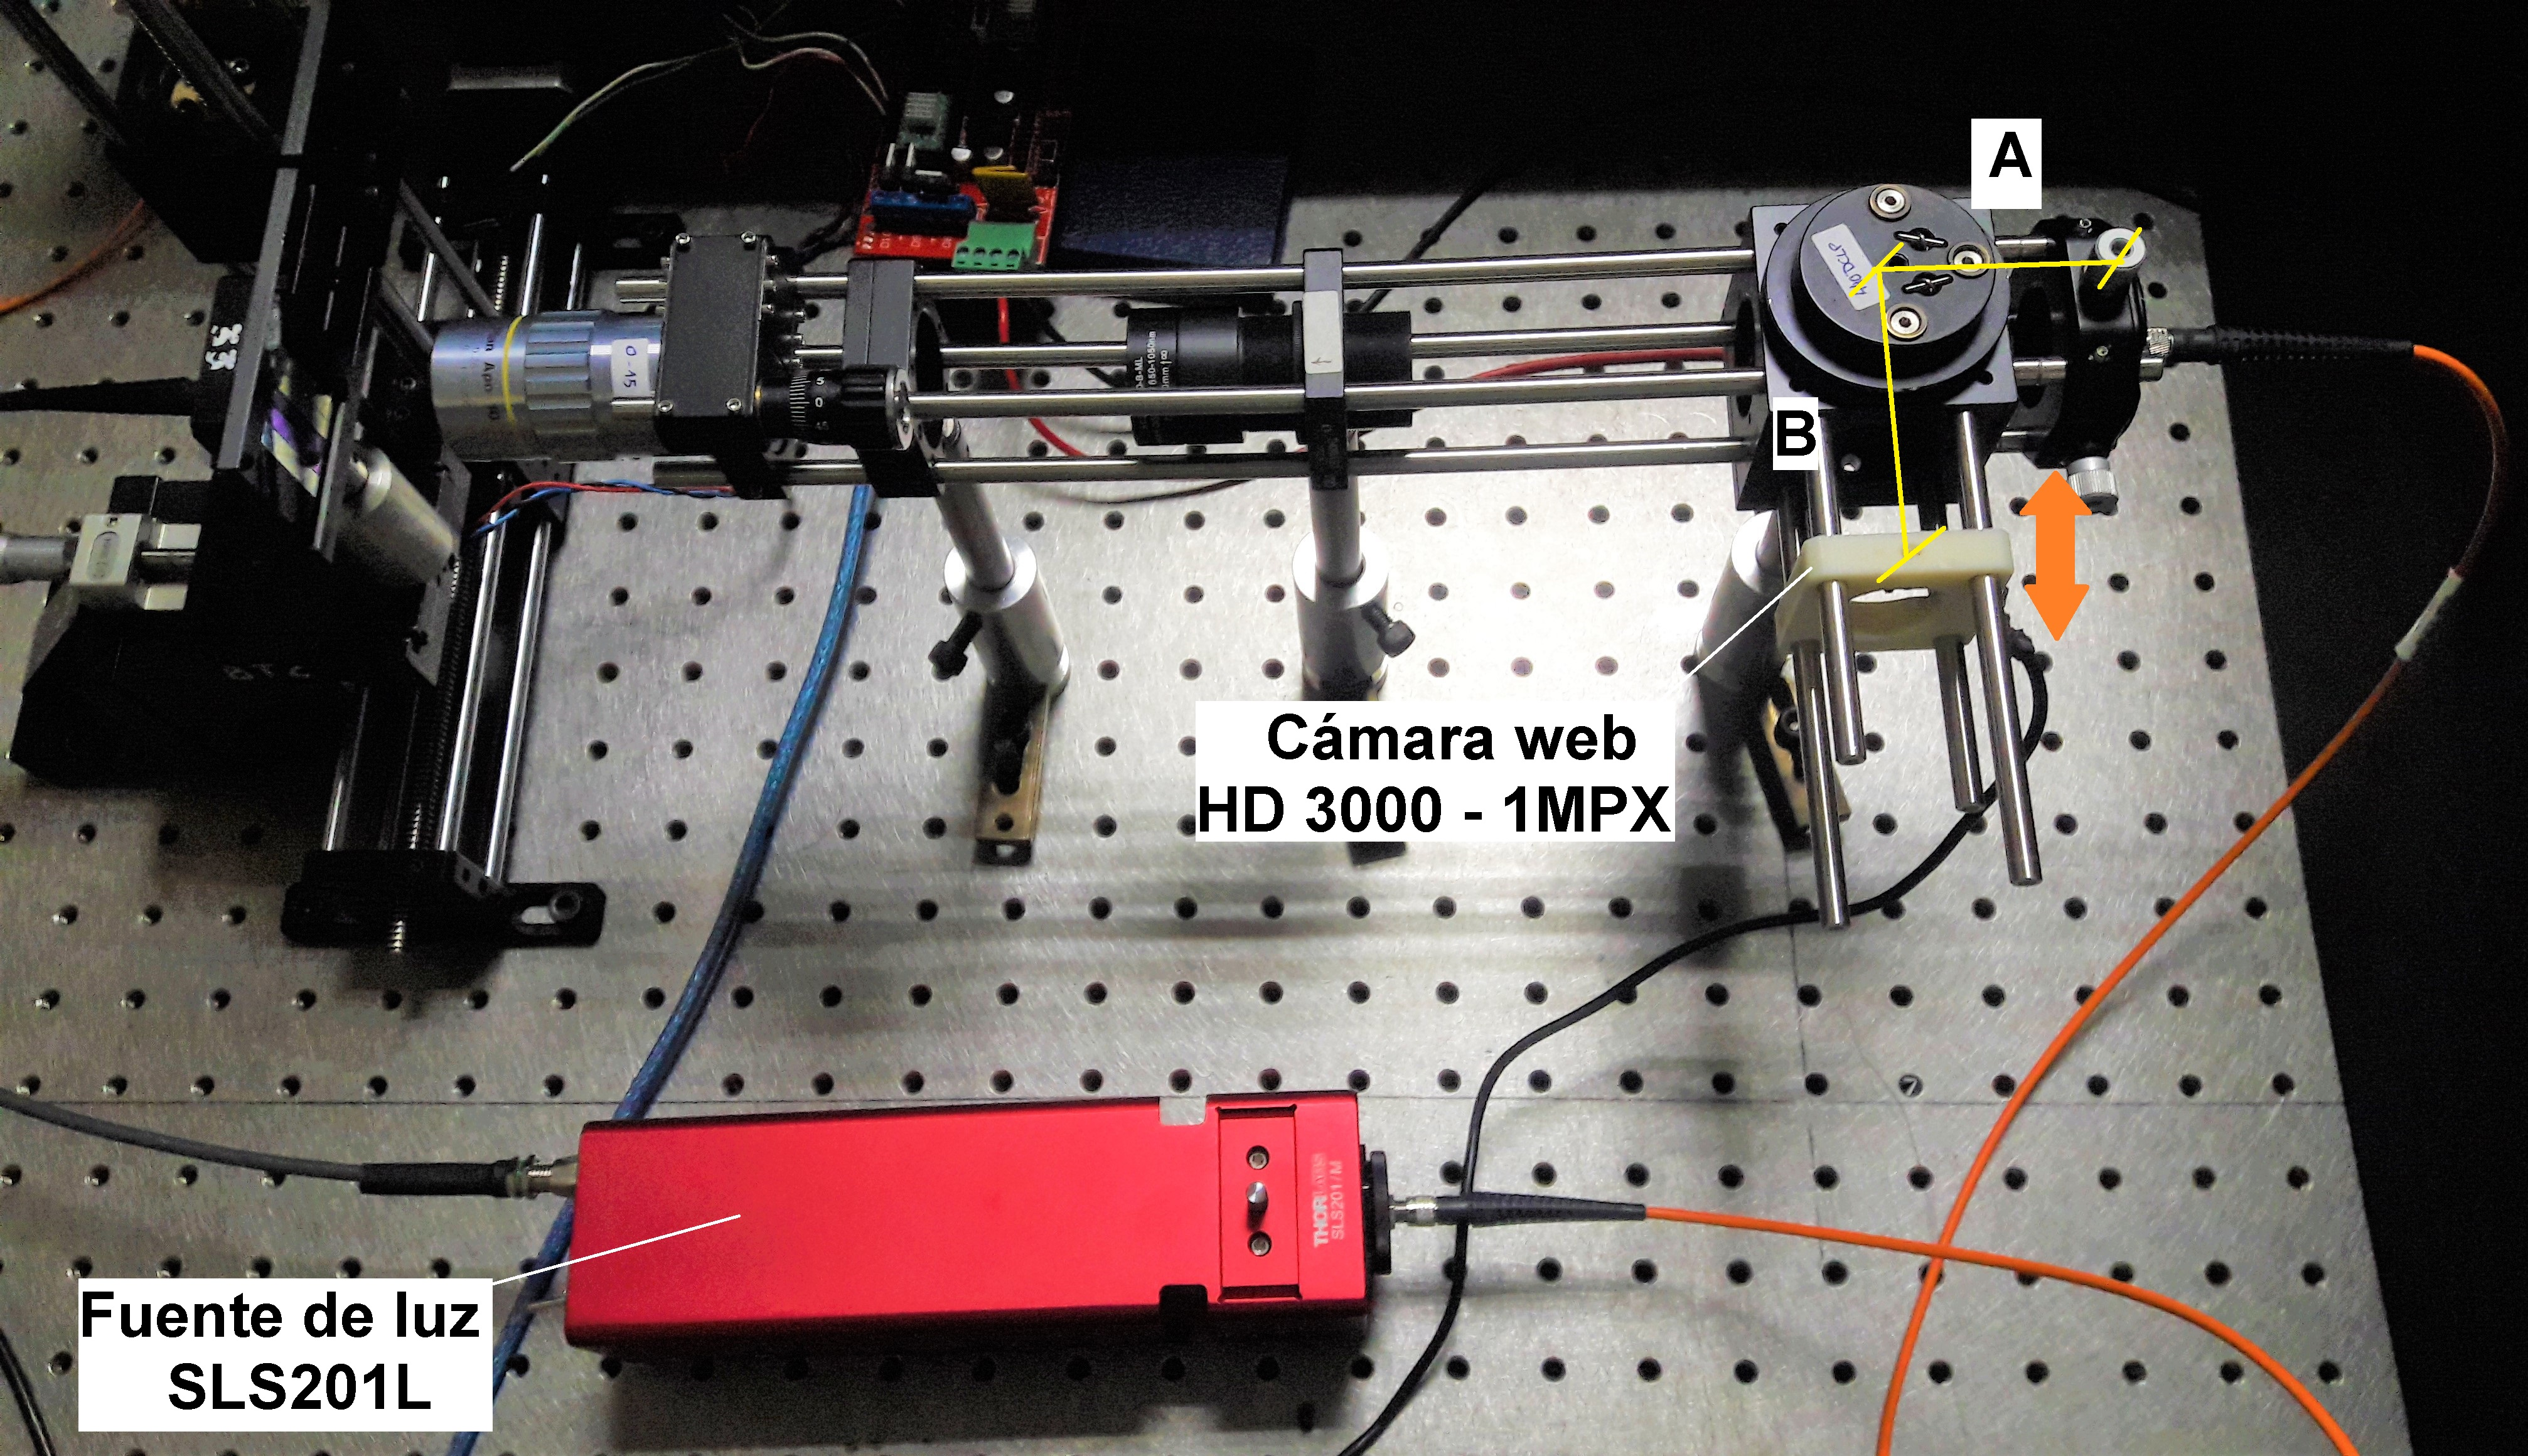
\includegraphics[scale=0.1]{Figs/microespectrometro/mapespeccam.jpg}
	\caption{Setup para mapear el espectrómetro con la cámara.}
	\label{fig:bgcel}
\end{figure}


Con los tornillos de la tapa de arriba del beamsplitter se puede ajustar en altura el beamsplitter para poder observar en el centro de la cámara la medición del espectrómetro.
\begin{figure}[H]
	\centering
	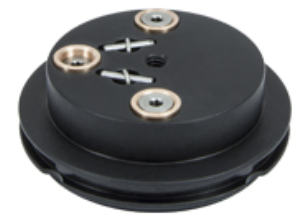
\includegraphics[scale=0.5]{Figs/microespectrometro/b4c.png}
	\caption{Tapa de arriba del beamsplitter.}
	\label{fig:bgcel}
\end{figure}


\begin{figure}[H]
	\centering
	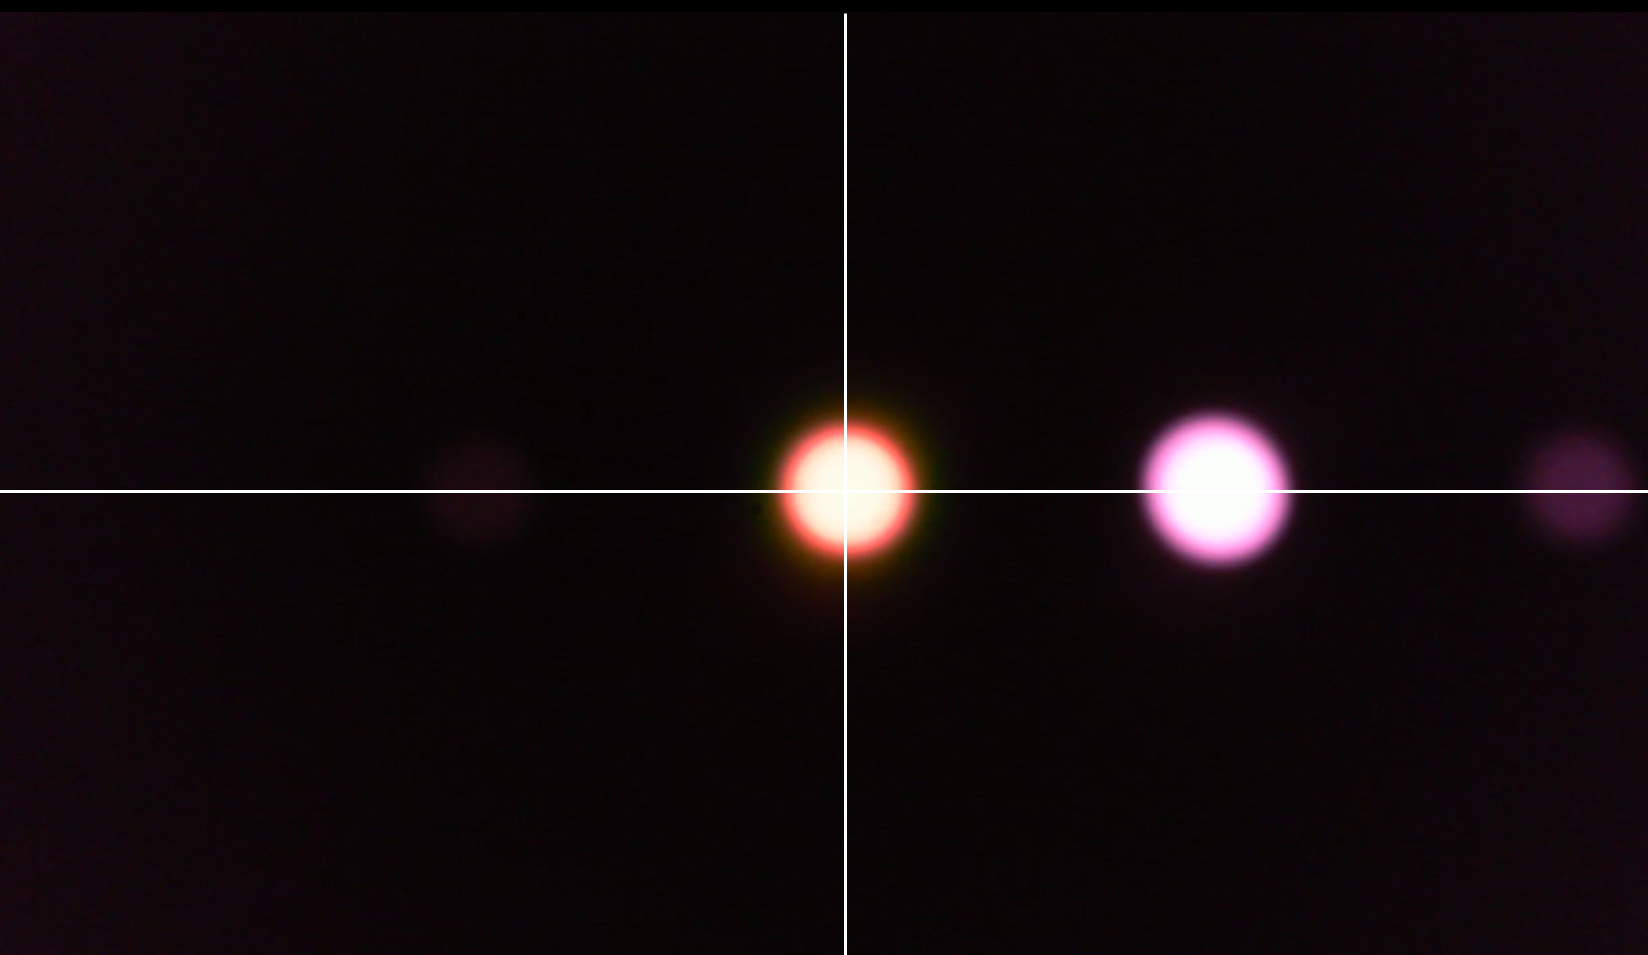
\includegraphics[scale=0.5]{Figs/microespectrometro/mapspectrometrocamera.png}
	\caption{Visualización en la cámara de la reflexión del filtro de la iluminación.}
	\label{fig:bgcel}
\end{figure}


No se tocó ni la cámara ni ninguna parte del setup a partir de ese momento para no perder este mapeo, a pesar de que la cámara no se encuentre perfectamente en foco (no hace falta probablemente poner una imagen de la cámara mostrando que no está en foco..), es decir que la imagen no se vea del todo nítida.
Luego se puso en foco el microespectrómetro.



\begin{figure}[H]
	\centering
	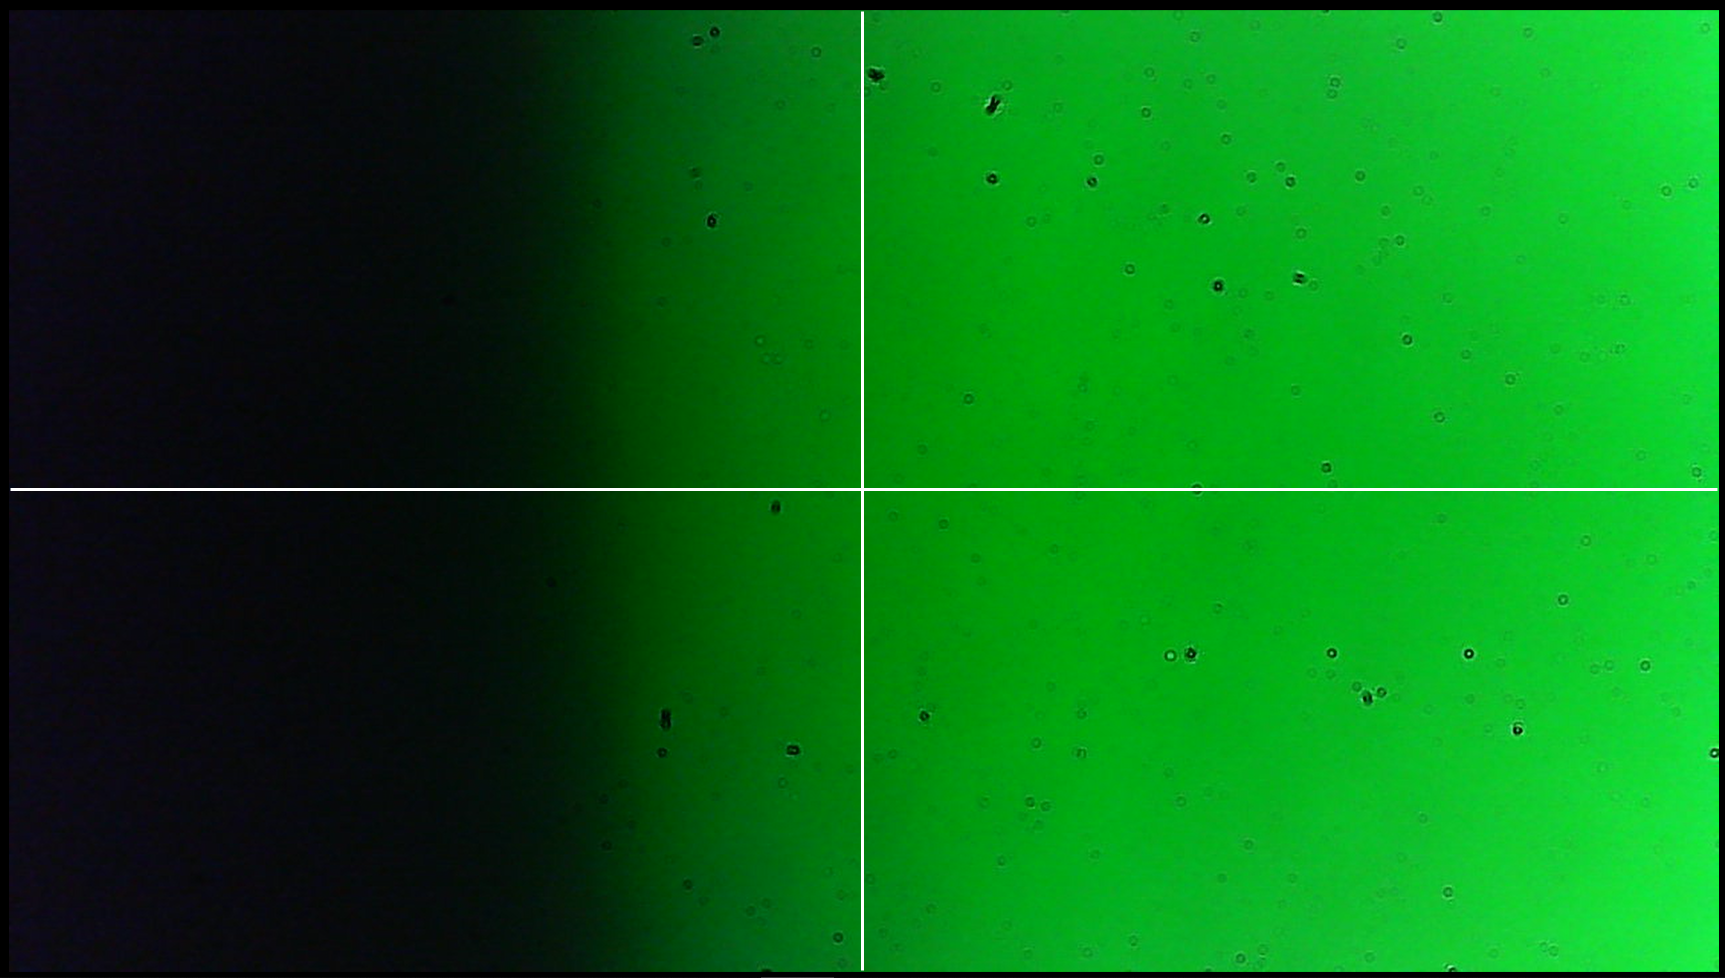
\includegraphics[scale=0.5]{Figs/microespectrometro/medtransicion.png}
	\caption{Visualización en la cámara de la reflexión del filtro de la iluminación.}
	\label{fig:bgcel}
\end{figure}


durante el experimento se tiene el feedback de cutelog:

\begin{figure}[H]
	\centering
	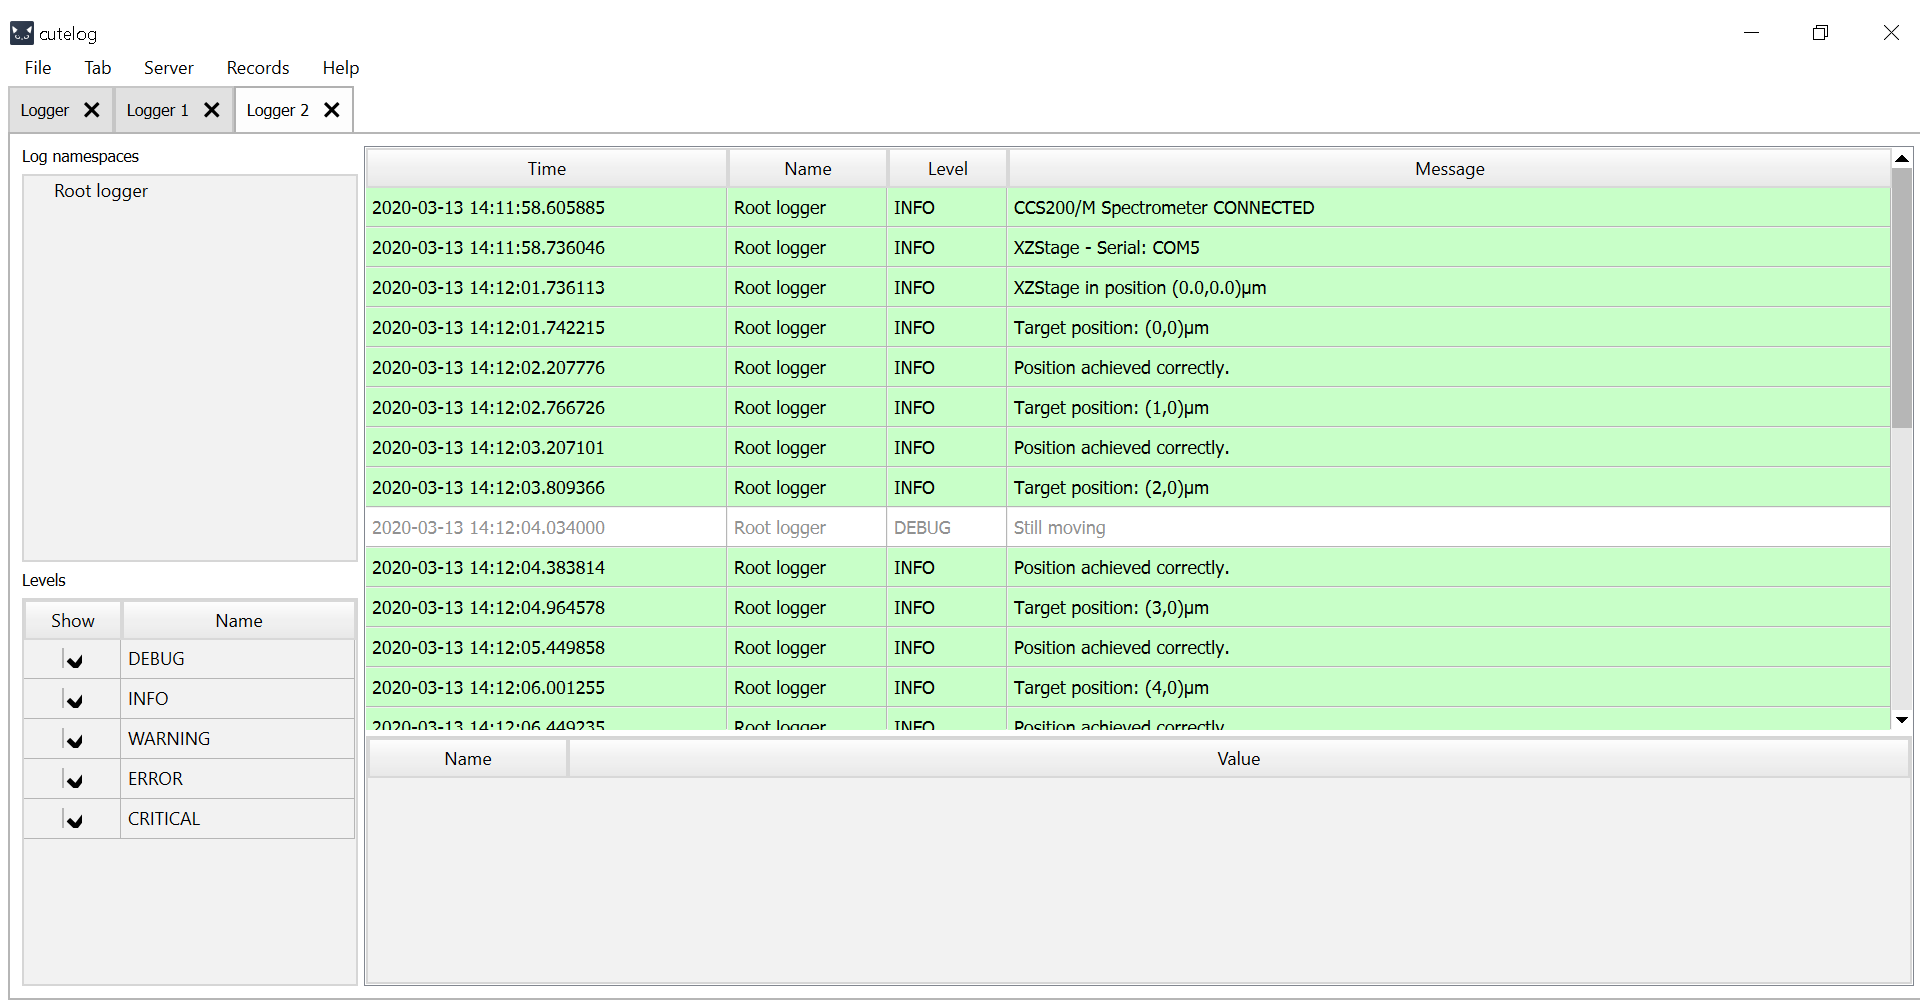
\includegraphics[scale=0.5]{Figs/microespectrometro/cutelog.png}
	\caption{Visualización en la cámara de la reflexión del filtro de la iluminación.}
	\label{fig:bgcel}
\end{figure}


\begin{figure}[H]
	\centering
	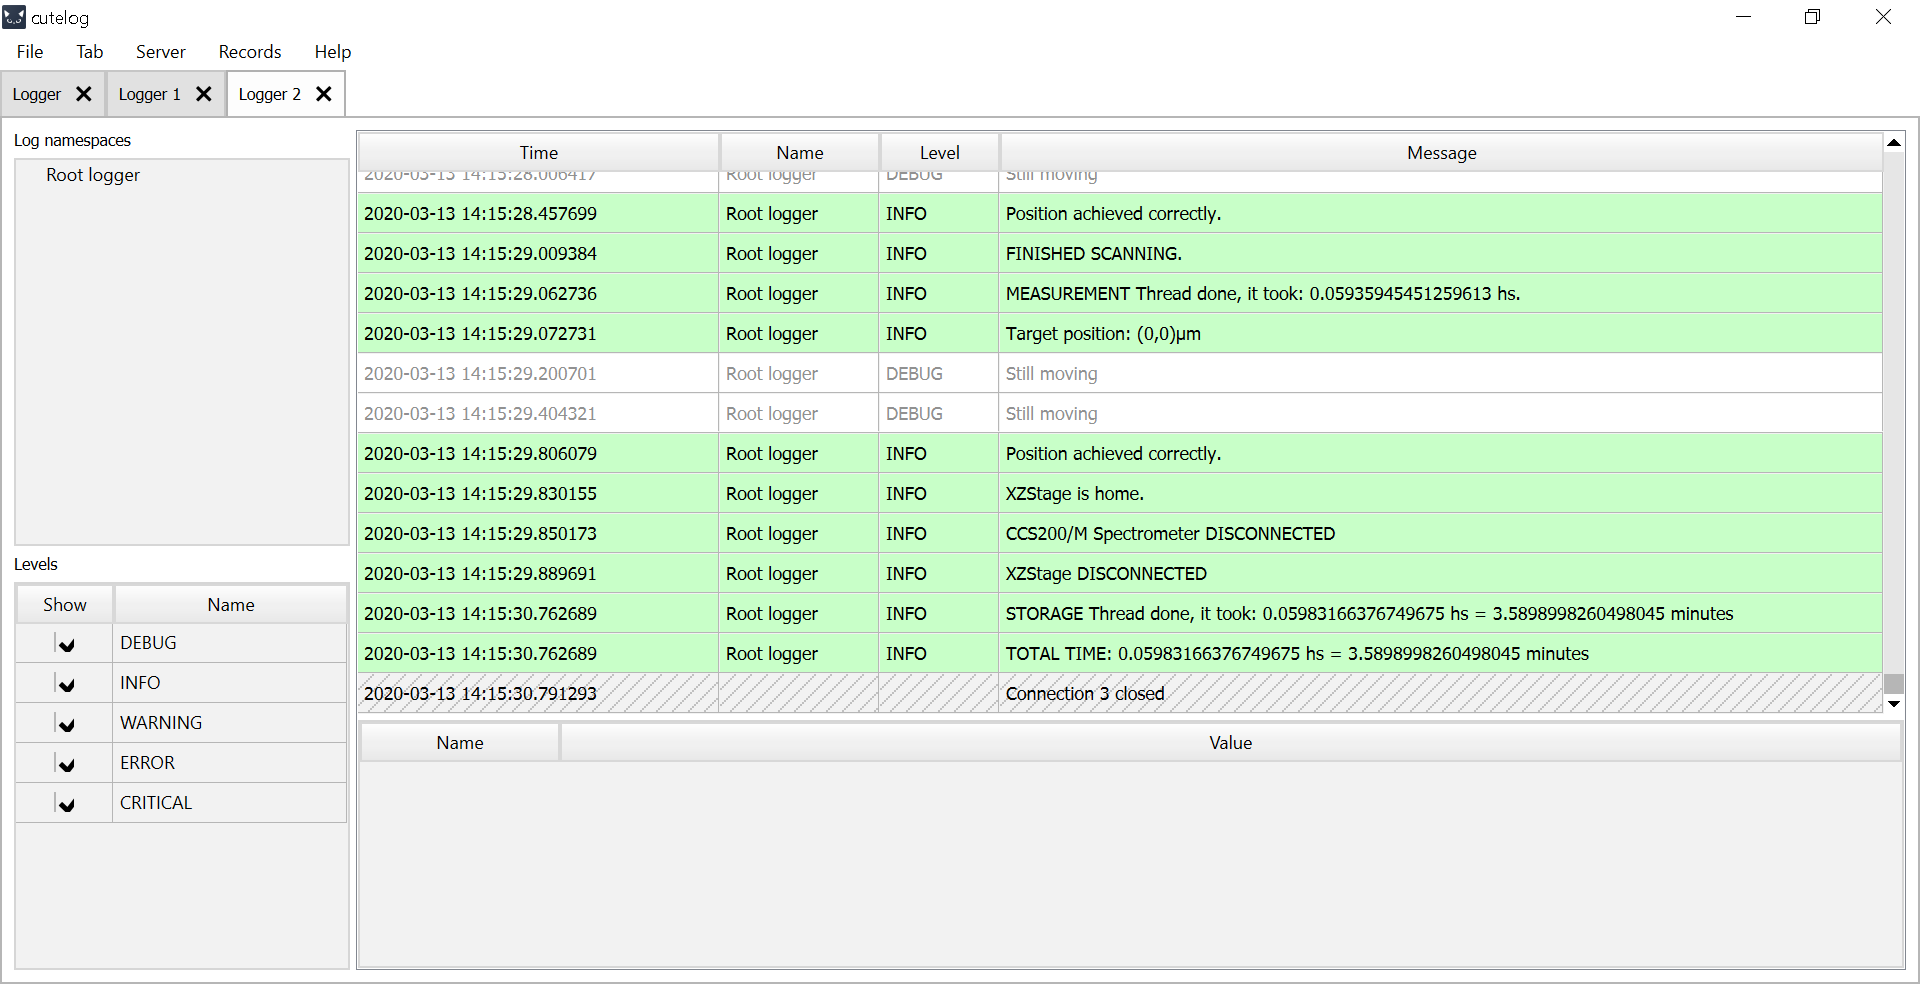
\includegraphics[scale=0.5]{Figs/microespectrometro/fincutelog.png}
	\caption{Visualización en la cámara de la reflexión del filtro de la iluminación.}
	\label{fig:bgcel}
\end{figure}


Las mediciones son ajustadas en matlab con una función error:
\begin{equation}
	(a/2)*erfc(sqrt(2)*(x-b)/c)
\end{equation}

\begin{figure}[H]
	\centering
	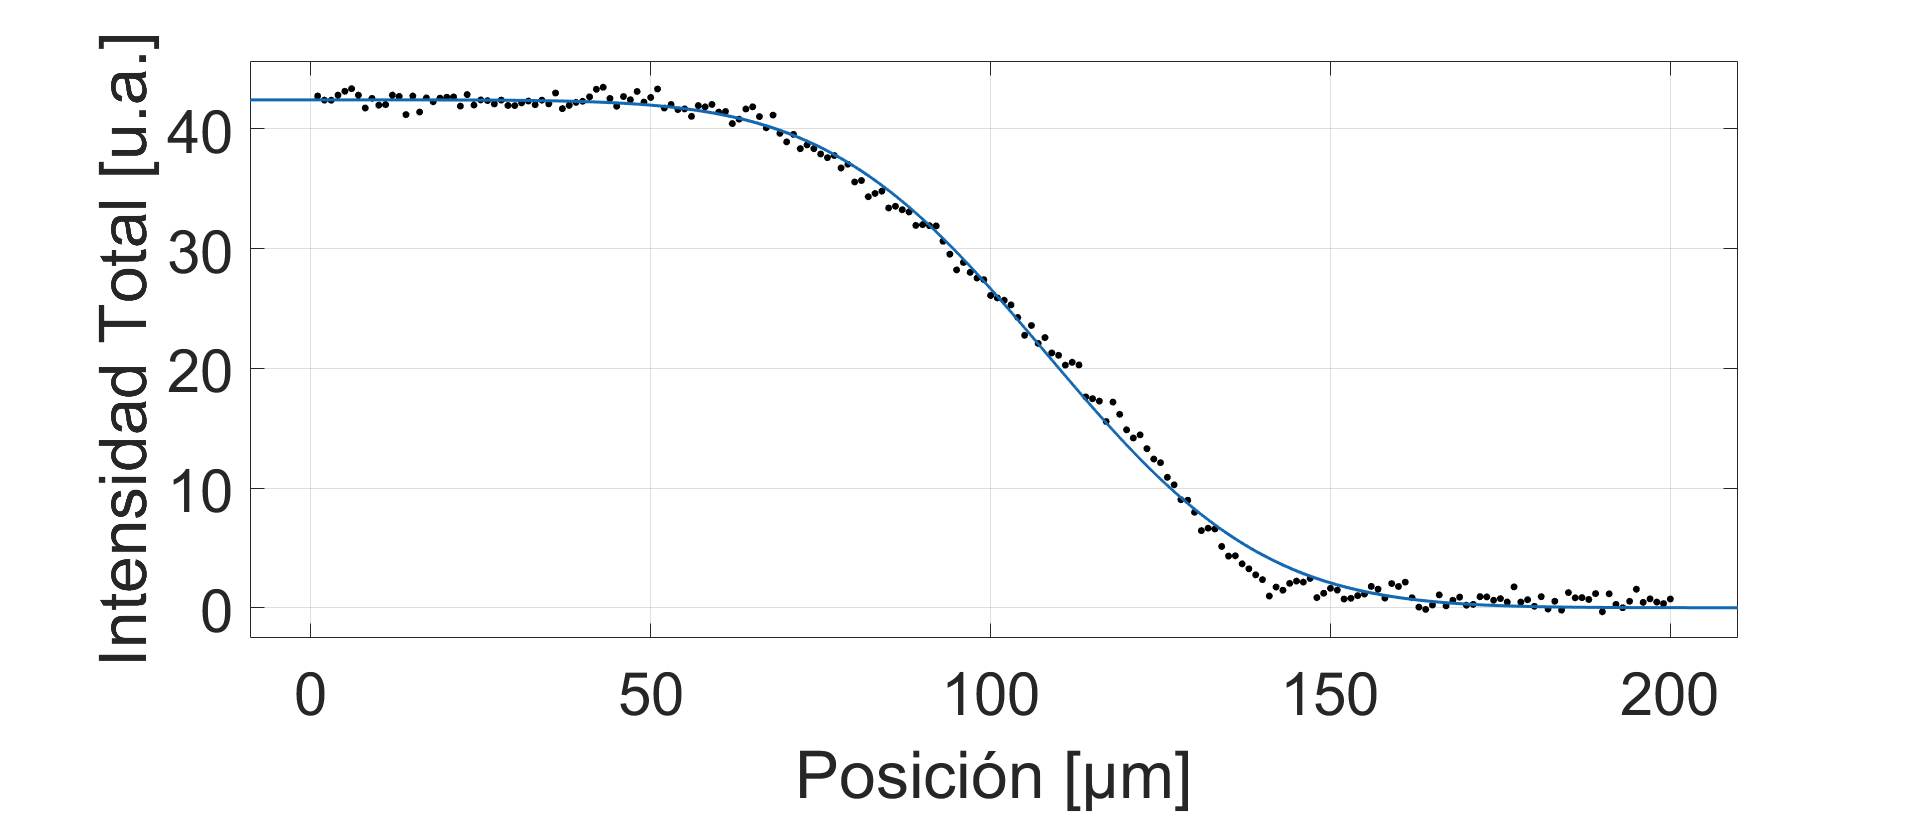
\includegraphics[scale=0.3]{Figs/microespectrometro/fit0.png}
	\caption{Visualización en la cámara de la reflexión del filtro de la iluminación.}
	\label{fig:bgcel}
\end{figure}

Resultados del ajuste:

General model:\par
$f(x) = (a/2)*erfc(sqrt(2)*(x-b)/c)$ \par
Coefficients (with 95$\%$ confidence bounds): \par
$a =       42.43  (42.2, 42.66)$\par
$b =       108.2  (107.8, 108.7)$\par
$c =       50.46  (49.25, 51.68)$\par

Goodness of fit:\par
SSE: 151.1\par
R-square: 0.9976\par
Adjusted R-square: 0.9976\par
RMSE: 0.8758\par

Luego moviendo la perilla del SM1Z para cambiar la distancia entre el objetivo y el filtro se repite la medición.


Comentar bien la siguiente foto, poner en la imagen que distancia se está variando, ettc
\begin{figure}[H]
	\centering
	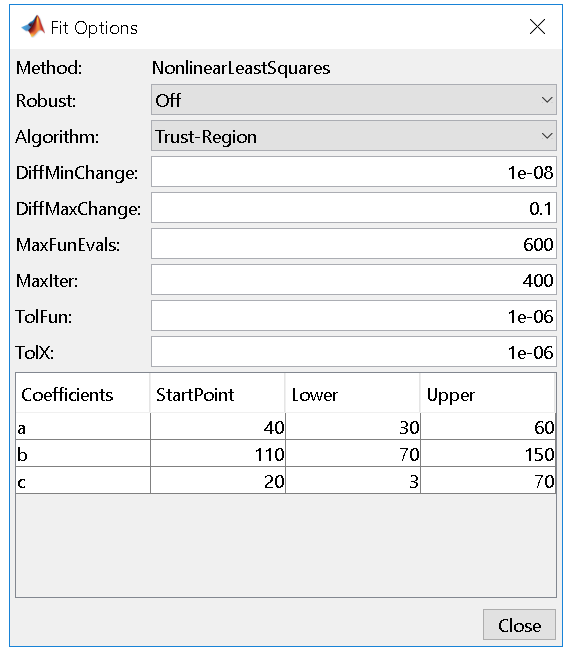
\includegraphics[scale=0.4]{Figs/microespectrometro/refinacionparam.png}
	\caption{Visualización en la cámara de la reflexión del filtro de la iluminación.}
	\label{fig:bgcel}
\end{figure}


Para hacer el ajuste se refinan los parámetros del modelo:

\begin{figure}[H]
	\centering
	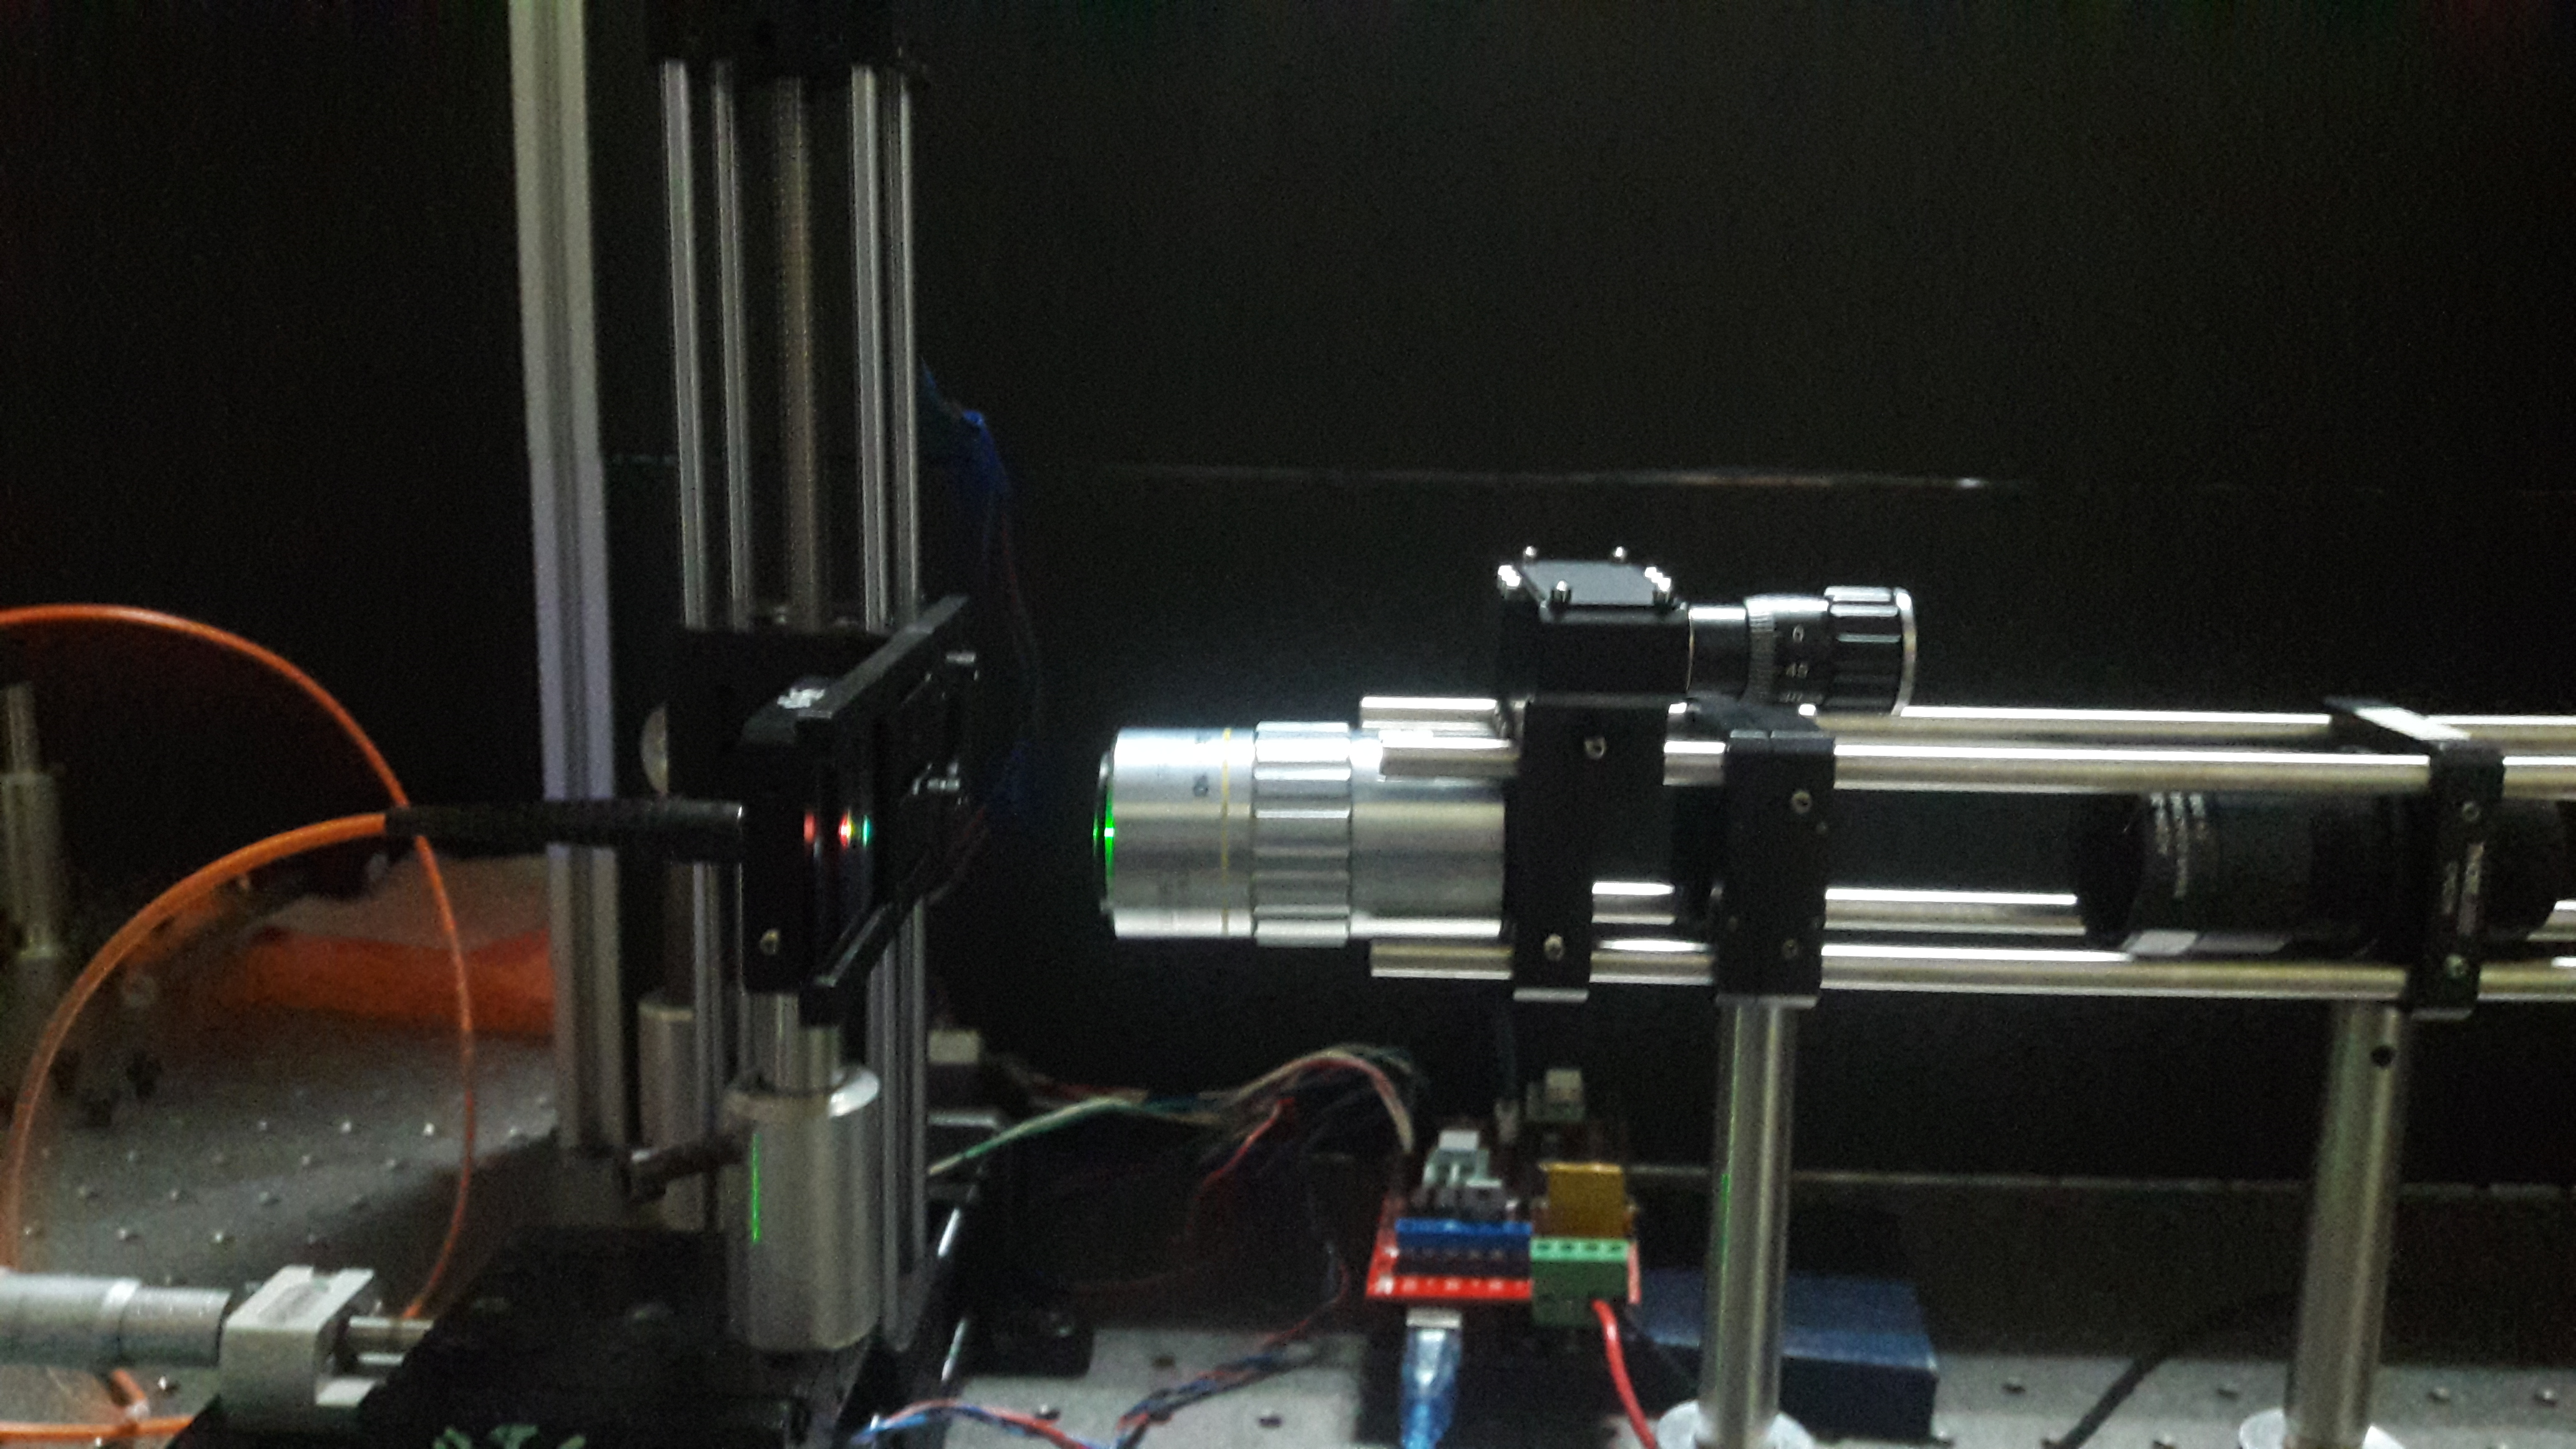
\includegraphics[scale=0.1]{Figs/microespectrometro/sm1zcambio.jpg}
	\caption{Visualización en la cámara de la reflexión del filtro de la iluminación.}
	\label{fig:bgcel}
\end{figure}


La idea es poner en foco el espectrómetro en alguna región del filtro, enfocar luego la cámara y después al mover el filtro a alguna otra región, tan solo hay que poner en foco el 'sistema' mirando la cámara. Al mismo tiempo si se quiere se puede volver a repetir el procedimiento de buscar el mínimo.


Gráfico de poner en foco el microespectrómetro: (19 de marzo)

mediciones guardadas en: data mediciones, simultaneidad, foco.

vamos recorriendo horario en pasos de 50 micrones en el SM1Z.
mediciones que consisten en un barrido de 80 micrones de largo, con pasos de 1 micron.. esto en la stage


RESULTADOS:

Z                  RESOLUCIÓN

0                  12.46 dudoso?

-50               13.5

-100             13.12

-150              12.87

-200              11.29



\singlespacing
\section{Integración de una cámara web}
\spacing{1.5}

\singlespacing
\subsection{Mapeando el espectrómetro con la cámara}
\spacing{1.5}